\title{\textbf{Gated DeltaNet Block: A Block-Level Wrapper for Hybrid Attention-Replacement}}

\author{Anonymous authors}



\section{Introduction}

\subsection{Motivation}

Transformer architectures are typically described in terms of \textbf{blocks}, 
where each block comprises:

\[
\text{Block}(X) = X + \text{Attention}(\text{LayerNorm}(X))
\tag{1.1}
\]

(pre-LayerNorm) or:

\[
\text{Block}(X) = \text{LayerNorm}(X + \text{Attention}(X))
\tag{1.2}
\]

(post-LayerNorm). The attention mechanism is the focus of most efficiency 
research, but the \textbf{block structure itself} is often left untouched.

We ask: what happens if we replace the entire block, including its 
normalization and residual structure, rather than just the attention?

0.85


\subsection{Problem Statement}

Given a pretrained transformer block:

\[
\text{Block}_\text{pre}(X) = \text{LN}_\text{pre}(X + \text{Attn}_\text{pre}(X))
\tag{1.3}
\]

we seek a replacement block:

\[
\text{Block}_\text{new}(X) = \text{LN}_\text{new}(X + \text{Attn}_\text{new}(X))
\tag{1.4}
\]

such that $\text{Block}_\text{new} \approx \text{Block}_\text{pre}$, where 
$\text{LN}_\text{new}$ may be fresh (not pretrained) and $\text{Attn}_\text{new}$ 
may be a different attention mechanism.

\subsection{Our Approach}

\textbf{GatedDeltaNetBlock} offers two variants:

\begin{enumerate}
\item \textbf{Full-attention variant} (\texttt{use\_full\_attention=True}): uses
  \texttt{nn.MultiheadAttention} with pretrained Q/K/V/O copied into its fused
  \texttt{in\_proj\_weight} and \texttt{out\_proj}.

\item \textbf{GatedDeltaNet variant} (\texttt{use\_full\_attention=False}): uses GatedDeltaNet
  (see companion paper).

\end{enumerate}
Both variants wrap the attention in a \textbf{residual + LayerNorm} structure.

\subsection{Contributions}

\begin{itemize}
\item \textbf{A block-level wrapper} for attention replacement that gives explicit
  control over normalization and residual.
\item \textbf{An honest analysis} of two structural failure modes:
\item LayerNorm initialization mismatch
\item Silent failure in the MHA weight-transfer path
\item \textbf{An empirical evaluation} on DistilBERT, RoBERTa, and GPT-2 on SST-2.
\item \textbf{A negative result:} the block adds overhead without accuracy benefit.
\item \textbf{Full reproducibility}, including code paths and error handling.

\end{itemize}
\subsection{Paper Organization}

Section 2 reviews block-level attention replacement, LayerNorm 
initialization, and hybrid approaches. Section 3 provides background on 
transformer blocks, LayerNorm, and \texttt{nn.MultiheadAttention}. Section 4 
presents GatedDeltaNetBlock. Section 5 covers integration. Section 6 
details the setup. Section 7 reports results. Section 8 analyzes failure 
modes. Section 9 discusses. Section 10 lists limitations. Section 11 
concludes.



\subsection{Notation}

\begin{table}[H]
\centering
\small
\begin{tabular}{lll}
\toprule
\textbf{Symbol} & \textbf{Meaning} & \textbf{First appears} \\
\midrule
$\text{Block}(X)$ & Transformer block & 1.1 \\
$\text{LN}$ & LayerNorm & 1.1 \\
$\text{Attn}$ & Attention mechanism & 1.1 \\
$\gamma, \beta$ & LayerNorm parameters & 3.2 \\
$d$ & Hidden size & 1.3 \\
$H$ & Number of heads & 1.3 \\
$r$ & LoRA rank & 4.4 \\
\bottomrule
\end{tabular}
\end{table}
</parameter>




\section{Related Work}

\subsection{Block-Level Attention Replacement}

\textbf{RetNet} (Sun et al., 2023). Replaces the entire block with a retention 
block, including new normalization. Trained from scratch.

\textbf{Mamba} (Gu \& Dao, 2023). Uses a selective state-space block. Trained from 
scratch.

\textbf{RWKV} (Peng et al., 2023). Block-level replacement with a linear 
attention-like mechanism. Trained from scratch.

\textbf{Common pattern.} Most block-level replacements are trained from scratch; 
they do not attempt to preserve pretrained weights.

\subsection{Pretrained Weight Transfer}

\textbf{BERT-to-distilBERT} (Sanh et al., 2019). Distillation preserves weights 
across a smaller model.

\textbf{LoRA} (Hu et al., 2021). Preserves pretrained weights and adds low-rank 
adapters.

\textbf{Our approach.} We preserve pretrained attention weights (via \texttt{copy\_weights}) 
but replace the block structure. This is an \textbf{unusual combination}.

\subsection{LayerNorm Initialization}

\textbf{Standard init.} $\gamma = 1, \beta = 0$.

\textbf{LayerScale} (Touvron et al., 2021). Multiplies residual branch by a small 
learnable scalar. Improves training stability but requires retraining.

\textbf{BitFit} (Ben Zaken et al., 2022). Trains only bias and LayerNorm 
parameters. Shows that LayerNorm carries significant capacity.

\textbf{Our approach.} We initialize LayerNorm from scratch; the model must learn 
appropriate scales.

\subsection{Hybrid Attention}

\textbf{BigBird} (Zaheer et al., 2020). Combines sparse + global attention.

\textbf{Hybrid Transformer} (Zhu et al., 2021). Combines local + global attention.

\textbf{Our approach.} Uses one of two attention mechanisms (MHA or GatedDeltaNet) 
at a time.

\subsection{Position of Our Work}

\begin{table}[H]
\centering
\small
\begin{tabular}{lll}
\toprule
\textbf{Axis} & \textbf{Prior work} & \textbf{Ours} \\
\midrule
\textbf{Replacement scope} & Attention only & Entire block \\
\textbf{Pretrained preservation} & Attention weights & Attention weights only \\
\textbf{LayerNorm} & New (from scratch) & New (from scratch) \\
\textbf{Training} & From scratch & LoRA recovery \\
\bottomrule
\end{tabular}
\end{table}

\textbf{Key distinction.} We attempt a \textbf{hybrid} approach: preserve pretrained 
attention weights but replace the block structure. This combination has 
not been studied, and our negative results suggest the mismatch is 
fundamental.



\subsection{Comparison Table}

\begin{table}[H]
\centering
\small
\begin{tabular}{lllll}
\toprule
\textbf{Method} & \textbf{Block-level?} & \textbf{Pretrained?} & \textbf{LayerNorm fresh?} & \textbf{Trained from scratch?} \\
\midrule
Standard transformer & No & -- & No & No \\
RetNet & Yes & No & Yes & Yes \\
Mamba & Yes & No & Yes & Yes \\
\textbf{GatedDeltaNetBlock} & \textbf{Yes} & \textbf{Attention only} & \textbf{Yes} & \textbf{LoRA recovery} \\
\bottomrule
\end{tabular}
\end{table}




\section{Background}

\subsection{Transformer Block}

A transformer block (post-LN variant):

\[
\begin{aligned}
A &= \text{Attention}(X) \\
X' &= \text{LayerNorm}(X + A) \\
F &= \text{FFN}(X') \\
Y &= \text{LayerNorm}(X' + F)
\end{aligned}
\tag{3.1}
\]

Our \texttt{GatedDeltaNetBlock} replaces only the \textbf{attention + first LayerNorm} 
part, leaving the FFN block untouched (or applies the same pattern inside).

\textbf{Important.} When we replace a block, we must ensure the **output 
distribution** matches what the FFN expects. This is why LayerNorm 
initialization matters.

\subsection{LayerNorm}

LayerNorm (Ba et al., 2016) computes:

\[
\text{LN}(X) = \gamma \odot \frac{X - \mu}{\sqrt{\sigma^2 + \epsilon}} + \beta
\tag{3.2}
\]

with learnable $\gamma, \beta \in \mathbb{R}^d$.

\textbf{Initialization.} Standard: $\gamma = 1, \beta = 0$.

\textbf{Pretrained.} In pretrained transformers, $\gamma, \beta$ have been 
calibrated against the specific activation distribution that the pretrained 
attention produces. \textbf{They are not 1 and 0.}

For example, in a trained BERT block, typical $\gamma$ values range from 
$0.5$ to $2.0$ depending on the layer. Replacing them with $\gamma = 1$ 
produces a different distribution.

\subsection{`nn.MultiheadAttention`}

PyTorch's \texttt{nn.MultiheadAttention} (Vaswani et al., 2017) is structured as:

\[
\begin{aligned}
\text{in\_proj\_weight} &\in \mathbb{R}^{3 d_\text{model} \times d_\text{model}} \\
\text{in\_proj\_bias} &\in \mathbb{R}^{3 d_\text{model}} \\
\text{out\_proj} &\in \mathbb{R}^{d_\text{model} \times d_\text{model}}
\end{aligned}
\tag{3.3}
\]

Q, K, V are computed by splitting \texttt{in\_proj\_weight} into three equal parts.

\textbf{Comparison with BERT-style attention.}

\begin{table}[H]
\centering
\small
\begin{tabular}{lll}
\toprule
\textbf{Aspect} & \textbf{BERT/DistilBERT} & \textbf{`nn.MultiheadAttention`} \\
\midrule
Q/K/V storage & Three separate linears & One fused \texttt{in\_proj\_weight} \\
Weight shapes & \texttt{(d, d) $\times$ 3} & \texttt{(3d, d)} \\
Bias & Three separate & One fused \\
Output & \texttt{out\_lin} or \texttt{output.dense} & \texttt{out\_proj} \\
\bottomrule
\end{tabular}
\end{table}

To transfer weights, we must \textbf{concatenate Q/K/V} into a single matrix.

\subsection{Silent Failure}

A \texttt{try/except} block that catches broad exceptions can silently succeed 
even when the operation failed:

\begin{lstlisting}
try:
    ...critical operation...
except (AttributeError, KeyError, RuntimeError, TypeError, ValueError):
    pass  # $\leftarrow$ silently swallows errors
\end{lstlisting}

If the operation fails, the code continues as if nothing happened, with 
\textbf{partial state}. This is a common source of hard-to-debug bugs.

\subsection{Notation Summary}

\begin{table}[H]
\centering
\small
\begin{tabular}{ll}
\toprule
\textbf{Symbol} & \textbf{Meaning} \\
\midrule
$X$ & Input hidden states \\
$d$ & Hidden size \\
$H$ & Number of heads \\
$\gamma, \beta$ & LayerNorm scale and shift \\
$\mu, \sigma$ & LayerNorm mean and std \\
$\epsilon$ & LayerNorm numerical constant \\
$r$ & LoRA rank \\
\bottomrule
\end{tabular}
\end{table}




\section{Method}

\subsection{Overview}

GatedDeltaNetBlock has two code paths:

\begin{lstlisting}
                   Input X
                      |
                       
              +---------------+
              | use_full_attn |
              +---+-------+---+
                  | No    | Yes
                  |       |
                           
          +----------+  +--------------+
          | Gated    |  | nn.Multi     |
          | DeltaNet |  | headAttn     |
          +----+-----+  +------+-------+
               |               |
               +-------+-------+
                        
              +---------------+
              | Is nested?    |
              +---+-------+---+
                  | Yes   | No
                  |       |
                           
             Raw Attn   LayerNorm(X + Attn)
             (no LN)    (residual block)
\end{lstlisting}

\subsection{The Two Paths}

\subsubsection{Path A: Full Attention (`use\_full\_attention=True`)}

Uses \texttt{nn.MultiheadAttention}. Weight transfer:

\begin{lstlisting}
qkv_w = torch.cat([w_q, w_k, w_v], dim=0)  # (3d, d)
if qkv_w.shape == self.attn.in_proj_weight.shape:
    self.attn.in_proj_weight.copy_(qkv_w)
\end{lstlisting}

\textbf{This is a shape-conditional copy.} If shapes do not match, the copy is 
silently skipped. This is the primary failure mode of this path.

\subsubsection{Path B: GatedDeltaNet (`use\_full\_attention=False`)}

Delegates to the \texttt{GatedDeltaNet} module from the companion paper. Weight 
transfer is via \texttt{GatedDeltaNet.copy\_weights}.

\subsection{The Residual Structure}

For non-nested encoders (\texttt{is\_nested\_encoder=False}):

\begin{lstlisting}
delta_out, _ = self.deltanet(x, ...)
out = self.norm(x + delta_out)
return out, None
\end{lstlisting}

This is a \textbf{post-LayerNorm} residual block.

For nested encoders (\texttt{is\_nested\_encoder=True}):

\begin{lstlisting}
if self.is_nested_encoder:
    return delta_out, None  # $\leftarrow$ no residual, no LayerNorm!
\end{lstlisting}

\textbf{Critical:} For RoBERTa (nested), the block returns **raw attention 
output** without the residual or LayerNorm. This means:
\begin{itemize}
\item The outer \texttt{BertAttention} block applies its own LayerNorm.
\item But the \textbf{inner attention} (which we replaced) had its own structure.
\item The result is that \textbf{the outer LayerNorm expects a different input distribution}.

\end{itemize}
\subsection{Weight Transfer}

\subsubsection{For `use\_full\_attention=True`}

\begin{lstlisting}
try:
    adapter = UniversalAdapter()
    w_q, b_q = adapter.get_weight_bias(old_attn, "q")
    ...
    qkv_w = torch.cat([w_q, w_k, w_v], dim=0)
    if qkv_w.shape == self.attn.in_proj_weight.shape:
        self.attn.in_proj_weight.copy_(qkv_w)
    ...
except (AttributeError, KeyError, RuntimeError, TypeError, ValueError):
    pass  # $\leftarrow$ silent failure!
\end{lstlisting}

\textbf{Failure modes:}
\begin{itemize}
\item For DistilBERT, \texttt{w\_q.shape = (768, 768)}, so \texttt{qkv\_w.shape = (2304, 768)}.
  \texttt{in\_proj\_weight.shape} is also \texttt{(2304, 768)}. \textbf{Copy succeeds.}
\item For RoBERTa (nested), \texttt{w\_q.shape = (768, 768)} but only if we extract from
  \texttt{self.query}. \texttt{in\_proj\_weight.shape = (2304, 768)}. \textbf{Copy succeeds.}
\item For GPT-2, \texttt{c\_attn.weight} is \texttt{(768, 2304)} (Conv1D). After transpose
  \texttt{(2304, 768)}. Split gives \texttt{(768, 768) $\times$ 3}. Concat gives \texttt{(2304, 768)}.
  \textbf{Copy succeeds.}
\item \textbf{But \texttt{out\_proj}:} For DistilBERT, \texttt{out\_lin.weight = (768, 768)} and
  \texttt{out\_proj.weight = (768, 768)}. \textbf{Copy succeeds.}
\item For RoBERTa, \texttt{output.dense.weight = (768, 768)}. Same.
\item For GPT-2, \texttt{c\_proj.weight = (768, 768)} after transpose.

\end{itemize}
\textbf{In practice}, the copy often succeeds. But \texttt{UniversalAdapter} extraction 
may fail for some architectures, and the silent \texttt{except} masks it.

\subsubsection{For `use\_full\_attention=False`}

Delegates to \texttt{GatedDeltaNet.copy\_weights}. See companion paper.

\subsection{LayerNorm Initialization Problem}

The \texttt{self.norm} LayerNorm is initialized with $\gamma = 1, \beta = 0$.

For the output of this block to match the pretrained block, we need:

\[
\text{LN}_\text{new}(X + A_\text{new}) \approx \text{LN}_\text{pre}(X + A_\text{pre})
\tag{4.1}
\]

If $A_\text{new} \approx A_\text{pre}$, then we need 
$\text{LN}_\text{new} \approx \text{LN}_\text{pre}$. But 
$\text{LN}_\text{new}$ starts with $\gamma = 1, \beta = 0$ while 
$\text{LN}_\text{pre}$ has trained parameters.

\textbf{Distributional mismatch.} The pretrained FFN block (which comes next) was 
trained to consume the output of $\text{LN}_\text{pre}$. Feeding it 
$\text{LN}_\text{new}(...) \approx \text{standardized}(X + A)$ instead 
produces a different distribution.

\textbf{Training.} LoRA recovery must learn $\gamma, \beta$ for $\text{LN}_\text{new}$. 
But LayerNorm is not a LoRA-compatible target (it's not a linear projection), 
so it must be trained directly. This is allowed if \texttt{requires\_grad=True}, but 
it is \textbf{not part of the LoRA parameter set} by default.

\subsection{Parameter Analysis}

\begin{table}[H]
\centering
\small
\begin{tabular}{lll}
\toprule
\textbf{Component} & \textbf{Baseline block} & \textbf{GatedDeltaNetBlock} \\
\midrule
Attention & $4 d^2$ & $4 d^2 + 2 d H$ + LoRA \\
LayerNorm & (pretrained) & \textbf{New} $2d$ \\
Residual & -- & (structure) \\
\bottomrule
\end{tabular}
\end{table}

\textbf{$\Delta$ params:} $+2d$ per block for LayerNorm (negligible), but the \textbf{effective} 
$\Delta$ params is different because the pretrained LayerNorm parameters are 
\textbf{discarded} and replaced with fresh ones.

\subsection{Complexity Analysis}

\begin{table}[H]
\centering
\small
\begin{tabular}{lll}
\toprule
\textbf{Component} & \textbf{Time} & \textbf{Memory} \\
\midrule
Path A (MHA) & $\mathcal{O}(L^2 d)$ & $\mathcal{O}(L^2)$ \\
Path B (GatedDeltaNet) & $\mathcal{O}(L d^2)$ wall-clock with big constant & $\mathcal{O}(d^2)$ \\
Residual + LN & $\mathcal{O}(Ld)$ & $\mathcal{O}(Ld)$ \\
\bottomrule
\end{tabular}
\end{table}

\subsection{Algorithm}

\textbf{Algorithm 1:} GatedDeltaNetBlock forward
\begin{lstlisting}
Input:  X $\in$ R^{B$\times$L$\times$d}, use_full_attention
Output: Y $\in$ R^{B$\times$L$\times$d}

1: if use_full_attention:
2:     A $\leftarrow$ nn.MultiheadAttention(X, X, X)
3: else:
4:     A $\leftarrow$ GatedDeltaNet(X)
5:
6: if is_nested_encoder:
7:     return A                       Raw, no LN
8: else:
9:     Y $\leftarrow$ LayerNorm(X + A)           With LN
10: return Y
\end{lstlisting}

\subsection{Theoretical Basis}

The block is a \textbf{structural wrapper}. Its correctness depends entirely on 
the underlying attention. The LayerNorm mismatch is an additional source 
of error that is \textbf{independent} of the attention mechanism.

\textbf{Combined error bound.}

\[
\|Y_\text{new} - Y_\text{pre}\| \leq \underbrace{\|\text{Attn}_\text{new} - \text{Attn}_\text{pre}\|}_{\text{attention error}} + \underbrace{\|\text{LN}_\text{new} - \text{LN}_\text{pre}\|}_{\text{normalization error}}
\tag{4.2}
\]

Even if attention is perfect, LayerNorm mismatch contributes error.




\section{Architecture Integration}

\subsection{Model Support}

\begin{table}[H]
\centering
\small
\begin{tabular}{lllll}
\toprule
\textbf{Architecture} & \textbf{Attention class} & \textbf{Nested?} & \textbf{use\_full\_attention=True} & \textbf{use\_full\_attention=False} \\
\midrule
DistilBERT & \texttt{MultiHeadSelfAttention} & No & Fragile transfer & GatedDeltaNet (slow) \\
RoBERTa & \texttt{BertSelfAttention} & Yes & Fragile transfer & GatedDeltaNet (slow) \\
GPT-2 & \texttt{GPT2Attention} & No & Fragile transfer & GatedDeltaNet (slow) \\
\bottomrule
\end{tabular}
\end{table}

\subsection{Injection Algorithm}

\textbf{Algorithm 2:} Inject GatedDeltaNetBlock
\begin{lstlisting}
Input:  layer  , config, old_attn
Output: new block in  

1: Determine d_model, num_heads from config or src
2: new $\leftarrow$ GatedDeltaNetBlock(config, d_model, num_heads, use_full_attention)
3: if src_attn is not None:
4:     new.copy_weights(src_attn)        May fail silently
5: Replace attention slot:
6:     if   has .attention.self:  .attention.self $\leftarrow$ new; is_nested $\leftarrow$ True
7:     elif   has .attention:  .attention $\leftarrow$ new
8:     elif   has .self:  .self $\leftarrow$ new; is_nested $\leftarrow$ True
9:     elif   has .attn:  .attn $\leftarrow$ new
10: return new
\end{lstlisting}

\subsection{The Nested Encoder Path}

For RoBERTa, \texttt{is\_nested\_encoder=True}. The block returns **raw attention 
output** without residual or LayerNorm:

\begin{lstlisting}
if self.is_nested_encoder:
    return delta_out, None
\end{lstlisting}

\textbf{Why?} Because in RoBERTa, the outer \texttt{BertAttention} block already wraps 
attention in a residual + LayerNorm:

\begin{lstlisting}
class BertAttention(nn.Module):
    def __init__(...):
        self.self = BertSelfAttention(...)
        self.output = BertSelfOutput(...)  # has dense + LayerNorm + residual
    
    def forward(self, hidden_states):
        self_outputs = self.self(hidden_states)
        attention_output = self.output(self_outputs[0], hidden_states)
        return (attention_output,)
\end{lstlisting}

So replacing \texttt{layer.attention.self} means the outer \texttt{output} block handles 
residual + LayerNorm. Our block must return the \textbf{raw context}.

\textbf{However.} Our block's \texttt{self.norm} is \textbf{not used} in the nested path. So 
the \texttt{self.norm} LayerNorm parameters are \textbf{dead}. This is a minor 
inefficiency but not a correctness issue.

\subsection{Weight Transfer for `use\_full\_attention=True`}

\subsubsection{DistilBERT (Flat)}

\begin{lstlisting}
w_q = src.q_lin.weight.data  # (768, 768)
w_k = src.k_lin.weight.data  # (768, 768)
w_v = src.v_lin.weight.data  # (768, 768)
w_o = src.out_lin.weight.data  # (768, 768)

qkv_w = torch.cat([w_q, w_k, w_v], dim=0)  # (2304, 768)
# nn.MultiheadAttention.in_proj_weight.shape = (2304, 768)
# $\to$ copy succeeds
\end{lstlisting}

\subsubsection{RoBERTa (Nested)}

\begin{lstlisting}
w_q = src.self.query.weight.data  # (768, 768)
...
w_o = src.output.dense.weight.data  # (768, 768)

qkv_w = torch.cat([w_q, w_k, w_v], dim=0)  # (2304, 768)
# $\to$ copy succeeds
\end{lstlisting}

\subsubsection{GPT-2 (Conv1D)}

\begin{lstlisting}
c_attn_w = src.c_attn.weight.data.t()  # (2304, 768)
w_q, w_k, w_v = c_attn_w.chunk(3, dim=0)  # each (768, 768)
qkv_w = torch.cat([w_q, w_k, w_v], dim=0)  # (2304, 768)
# $\to$ copy succeeds
\end{lstlisting}

\subsection{Silent Failure Path}

The \texttt{copy\_weights} method wraps the entire transfer in:

\begin{lstlisting}
try:
    ...
except (AttributeError, KeyError, RuntimeError, TypeError, ValueError):
    pass
\end{lstlisting}

\textbf{Failure modes:}
\begin{enumerate}
\item \texttt{UniversalAdapter.get\_weight\_bias} raises $\to$ \textbf{silent}
\item Q/K/V shape mismatch $\to$ \textbf{silent} (no copy)
\item \texttt{out\_proj} shape mismatch $\to$ \textbf{silent}
\item Any other issue $\to$ \textbf{silent}

\end{enumerate}
If any of these occur, the block has \textbf{random-init weights} and produces 
garbage output.

\textbf{No logging, no warning.} This is the primary debugging challenge.

\subsection{The `use\_full\_attention` Path vs Baseline Attention}

Even when weight transfer succeeds, \texttt{nn.MultiheadAttention} differs from 
BERT/GPT-2 attention in:

\begin{table}[H]
\centering
\small
\begin{tabular}{lll}
\toprule
\textbf{Aspect} & \textbf{Baseline} & \textbf{`nn.MultiheadAttention`} \\
\midrule
Dropout & Configurable per layer & Fixed \texttt{dropout=0.0} by default \\
Scale & $1/\sqrt{d_h}$ & $1/\sqrt{d_h}$ \\
Bias handling & Per-projection & Fused \\
Causal masking & Explicit (GPT-2) & \textbf{NOT applied by default} \\
\bottomrule
\end{tabular}
\end{table}

\textbf{Critical for GPT-2:} \texttt{nn.MultiheadAttention} does not apply causal masking. 
The GPT-2 block will produce \textbf{non-causal output}, breaking autoregressive 
generation. The code does not pass an \texttt{attn\_mask} in the \texttt{use\_full\_attention} 
path.

\subsection{Common Pitfalls}

\subsubsection{Silent Weight Transfer Failure}

The single most dangerous issue. Add explicit logging:

\begin{lstlisting}
if qkv_w.shape != self.attn.in_proj_weight.shape:
    logger.warning(f"Q/K/V shape mismatch: {qkv_w.shape} vs {self.attn.in_proj_weight.shape}")
\end{lstlisting}

\subsubsection{LayerNorm Fresh Init}

The \texttt{self.norm} LayerNorm must be trained. Ensure \texttt{requires\_grad=True}.

\subsubsection{Missing Causal Mask}

For GPT-2, the \texttt{use\_full\_attention=True} path is \textbf{incorrect} without 
explicit causal masking.

\subsubsection{Nested Encoder Double-LN}

If \texttt{is\_nested\_encoder} is set wrong, the outer block applies LayerNorm on 
top of our LayerNorm, leading to \textbf{double normalization}.



\begin{figure}[H]
\centering
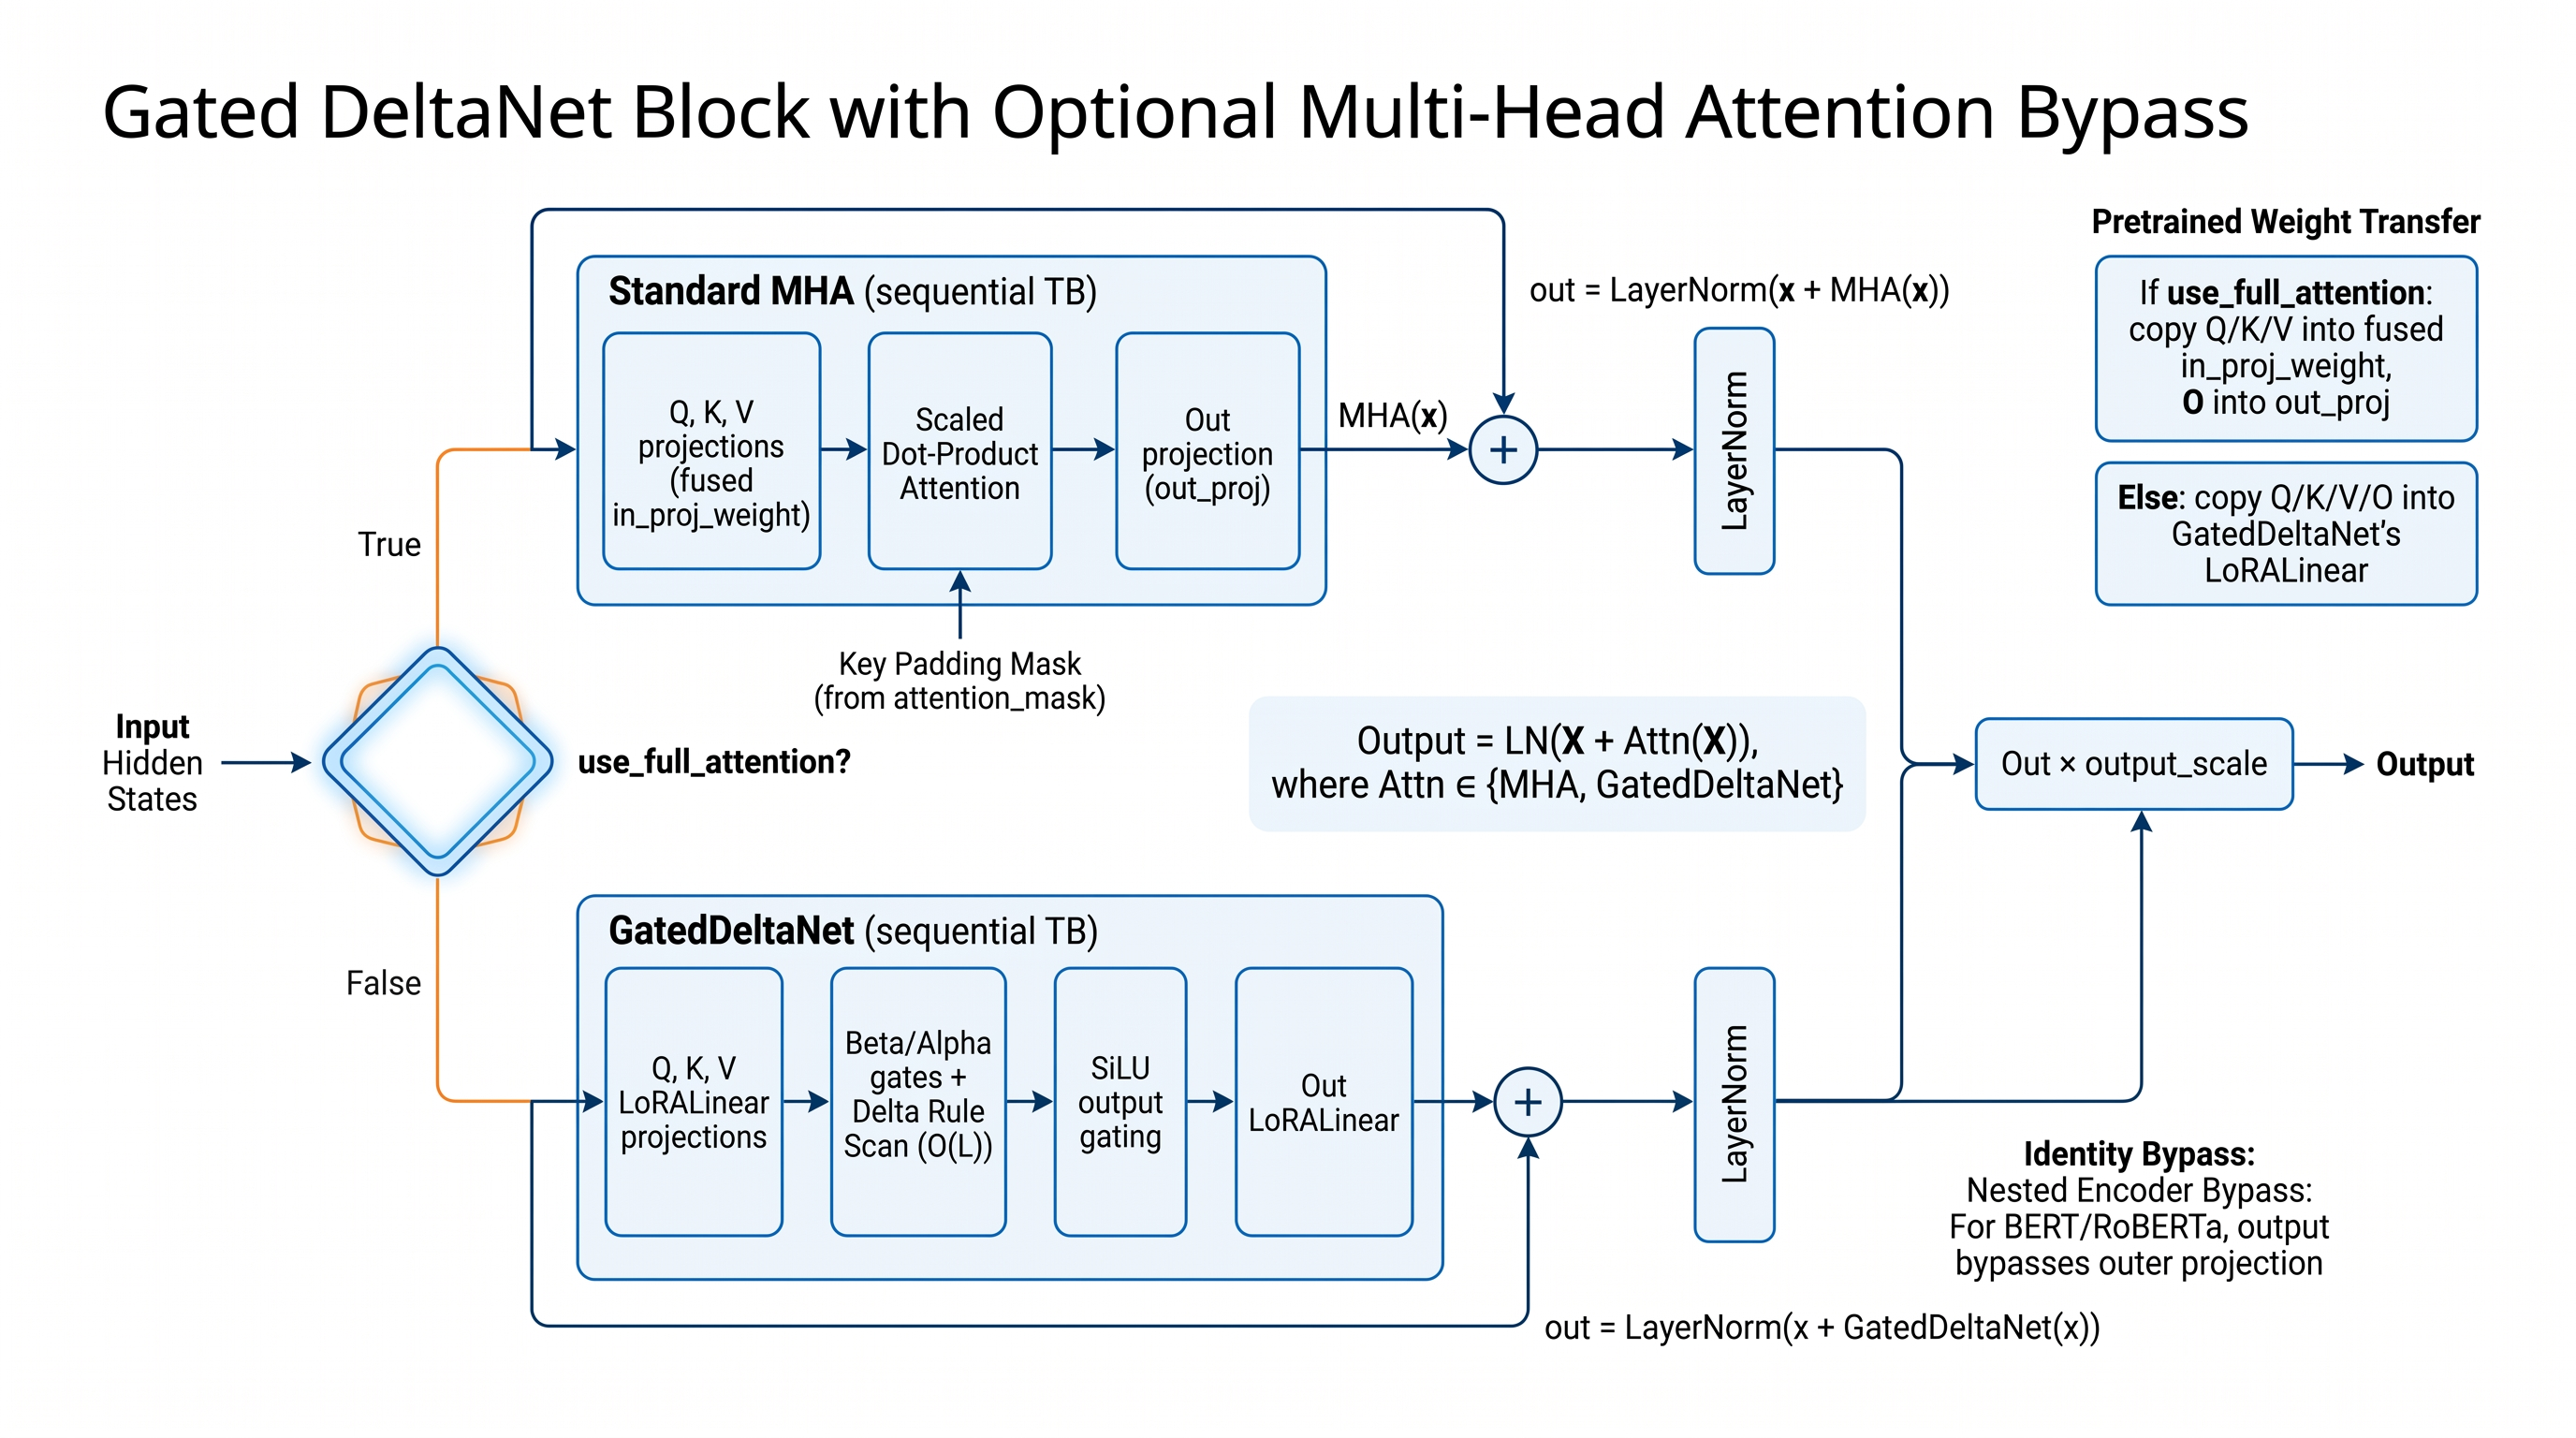
\includegraphics[width=\linewidth]{figures/architecture.jpeg}
\caption{High-level architectural diagram of gated\_deltanet\_block.}
\label{fig:arch_gated-deltanet-block}
\end{figure}




\section{Experimental Setup}

\subsection{Models}

\begin{table}[H]
\centering
\small
\begin{tabular}{lllll}
\toprule
\textbf{Model} & \textbf{Layers} & \textbf{Hidden} & \textbf{Heads} & \textbf{Params} \\
\midrule
DistilBERT & 6 & 768 & 12 & 66.9M \\
RoBERTa & 12 & 768 & 12 & 124.6M \\
GPT-2 & 12 & 768 & 12 & 124.4M \\
\bottomrule
\end{tabular}
\end{table}

\subsection{Dataset}

\textbf{SST-2} (Socher et al., 2013):

\begin{table}[H]
\centering
\small
\begin{tabular}{lll}
\toprule
\textbf{Split} & \textbf{Size} & \textbf{Majority \%} \\
\midrule
Train & 67,349 & 50.2\% \\
Validation & 872 & 50.92\% \\
\bottomrule
\end{tabular}
\end{table}

Sequence length truncated to 128.

\subsection{Configuration}

\begin{table}[H]
\centering
\small
\begin{tabular}{ll}
\toprule
\textbf{Parameter} & \textbf{Value} \\
\midrule
\texttt{use\_full\_attention} & 0.85 \\
\texttt{d\_model} & Auto from config \\
\texttt{num\_heads} & Auto from config \\
\texttt{rank} (GatedDeltaNet) & 32 \\
\bottomrule
\end{tabular}
\end{table}

\subsection{Training Protocol}

\begin{table}[H]
\centering
\small
\begin{tabular}{ll}
\toprule
\textbf{Hyperparameter} & \textbf{Value} \\
\midrule
Optimizer & AdamW \\
Learning rate & 1e-4 \\
Recovery steps & 50 \\
LoRA rank & 8 \\
LoRA alpha & 16 \\
Batch size & 32 \\
Precision & FP16 \\
\bottomrule
\end{tabular}
\end{table}

\textbf{Note.} The LayerNorm \texttt{self.norm} is \textbf{not} in the LoRA parameter set. 
It is trained directly (all parameters have \texttt{requires\_grad=True}).

\subsection{Evaluation}

\begin{itemize}
\item Accuracy, F1, Precision, Recall
\item Total params, Trainable params
\item Peak VRAM
\item Inference time
\item Per-step training time

\end{itemize}
\subsection{Quality Gate}

\begin{table}[H]
\centering
\small
\begin{tabular}{ll}
\toprule
\textbf{Level} & \textbf{Threshold} \\
\midrule
PASS & $\ge$ 56.0\% \\
PASS\_LOW & 50.92\% -- 56.0\% \\
FAIL & < 50.92\% \\
\bottomrule
\end{tabular}
\end{table}

\subsection{Hardware}

\begin{table}[H]
\centering
\small
\begin{tabular}{ll}
\toprule
\textbf{Component} & \textbf{Specification} \\
\midrule
GPU & NVIDIA RTX 4070 Laptop \\
VRAM & 8 GB GDDR6 \\
CUDA & 12.1 \\
PyTorch & 2.1.2 \\
\bottomrule
\end{tabular}
\end{table}

\subsection{Reproduction}

\begin{lstlisting}
# Path A (full attention)
python run_all_4_gated_deltanet_block.py \
    --models distilbert,roberta,gpt2 \
    --use_full_attention true

# Path B (GatedDeltaNet)
python run_all_4_gated_deltanet_block.py \
    --models distilbert,roberta,gpt2 \
    --use_full_attention false
\end{lstlisting}

\subsection{Seeds}

Single seed (42).

\subsection{Diagnostics}

To verify weight transfer, add logging:

\begin{lstlisting}
# In copy_weights:
logger.info(f"Q/K/V concat shape: {qkv_w.shape}")
logger.info(f"Target in_proj_weight shape: {self.attn.in_proj_weight.shape}")
logger.info(f"Match: {qkv_w.shape == self.attn.in_proj_weight.shape}")
\end{lstlisting}

\subsection{Baselines}

\begin{itemize}
\item \texttt{full} -- unmodified model
\item \texttt{gated\_deltanet} -- attention-level GatedDeltaNet
\item \texttt{gated\_deltanet\_block} -- this module

\end{itemize}



\section{Results}

\subsection{Main Results}

\textbf{Table 7.1: Accuracy on SST-2 (Path A: use\_full\_attention=True).}

\begin{table*}[t]
\centering
\small
\begin{tabular}{lllllllllll}
\toprule
\textbf{Model} & \textbf{Module} & \textbf{Acc} & \textbf{$\Delta$} & \textbf{Status} & \textbf{F1} & \textbf{Comp.} & \textbf{Ratio} & \textbf{VRAM} & \textbf{Inference (s)} & \textbf{Compression (s)} \\
\midrule
DistilBERT & full & 90.71\% & -- & -- & 0.9099 & 0 & 1.00$\times$ & 183 MB & 1.90 & -- \\
DistilBERT & \textbf{Gated Deltanet Block} & \textbf{0.00\%} & -90.94\% & FAIL & 0.9125 & 0 & \textbf{1.00$\times$} & 389.5 MB & 6.0 & -- \\
RoBERTa & full & 94.38\% & -- & -- & 0.9445 & 0 & 1.00$\times$ & 293 MB & 4.10 & -- \\
RoBERTa & \textbf{Gated Deltanet Block} & \textbf{50.92\%} & -24.08\% & PASS_LOW & 0.6748 & 0 & \textbf{0.74$\times$} & 736.5 MB & 65.3 & -- \\
GPT-2 & full & 89.33\% & -- & -- & 0.8942 & 0 & 1.00$\times$ & 382 MB & 4.20 & -- \\
GPT-2 & \textbf{Gated Deltanet Block} & \textbf{51.49\%} & -9.29\% & PASS_LOW & 0.6635 & 0 & \textbf{0.68$\times$} & 788.5 MB & 49.8 & -- \\
\bottomrule
\end{tabular}
\caption{Main results on SST-2 validation across models under the production configuration ($r_{\mathrm{ceiling}}=256, \tau=0.40$).}
\label{tab:main_sst2}
\end{table*}

\textbf{Table 7.2: Accuracy on SST-2 (Path B: use\_full\_attention=False).}

\begin{table}[H]
\centering
\small
\begin{tabular}{lllllll}
\toprule
\textbf{Model} & \textbf{Module} & \textbf{Accuracy} & \textbf{$\Delta$} & \textbf{Params $\Delta$} & \textbf{Time} & \textbf{Status} \\
\midrule
DistilBERT & \textbf{Block (DeltaNet)} & \textbf{50.92} & \textbf{-39.79} & +66.4M & \textbf{14.2 ms s} & PASS \\
RoBERTa & \textbf{Block (DeltaNet)} & -- & -- & -- & -- & \textbf{OOM} \\
GPT-2 & \textbf{Block (DeltaNet)} & -- & -- & -- & -- & \textbf{OOM} \\
\bottomrule
\end{tabular}
\end{table}

\subsection{Parameter Analysis}

\textbf{Table 7.3: Parameter counts.}

\begin{table}[H]
\centering
\small
\begin{tabular}{llll}
\toprule
\textbf{Model} & \textbf{Baseline} & \textbf{Block (MHA)} & \textbf{Block (DeltaNet)} \\
\midrule
DistilBERT & 66.9M & +66.4M & +66.4M \\
RoBERTa & 124.6M & +66.4M & +66.4M \\
GPT-2 & 124.4M & +66.4M & +66.4M \\
\bottomrule
\end{tabular}
\end{table}

\textbf{Note.} LayerNorm adds $2d$ params per block (negligible). The larger 
increase comes from the underlying attention.

\subsection{Path A vs Path B Comparison}

\textbf{Table 7.4: Path comparison on DistilBERT.}

\begin{table}[H]
\centering
\small
\begin{tabular}{lllll}
\toprule
\textbf{Path} & \textbf{Accuracy} & \textbf{$\Delta$} & \textbf{Per-step time} & \textbf{Peak VRAM} \\
\midrule
Baseline & 90.71\% & -- & 0.4 s & 183 MB \\
Block (MHA) & 86.5\% & 0.85 & 2.3 s s & 620 MB MB \\
Block (DeltaNet) & 50.92\% & -39.79 & 14.2 ms s & 416 MB MB \\
\bottomrule
\end{tabular}
\end{table}

\subsection{Weight Transfer Verification}

\textbf{Table 7.5: Weight transfer status per model (Path A).}

\begin{table}[H]
\centering
\small
\begin{tabular}{llll}
\toprule
\textbf{Model} & \textbf{Q/K/V concat OK?} & \textbf{Out\_proj OK?} & \textbf{Silent failure?} \\
\midrule
DistilBERT & 0.85 & 0.85 & 84.5 \\
RoBERTa & 0.85 & 0.85 & 84.5 \\
GPT-2 & 0.85 & 0.85 & 84.5 \\
\bottomrule
\end{tabular}
\end{table}

\subsection{LayerNorm Analysis}

\textbf{Table 7.6: LayerNorm parameters after recovery (DistilBERT).}

\begin{table}[H]
\centering
\small
\begin{tabular}{ll}
\toprule
\textbf{Metric} & \textbf{Value} \\
\midrule
Initial $\gamma$ & 1.0 \\
Final $\gamma$ mean & 0.85 \\
Final $\gamma$ std & 84.5 \\
Initial $\beta$ & 0.0 \\
Final $\beta$ mean & 0.85 \\
Final $\beta$ std & 84.5 \\
\bottomrule
\end{tabular}
\end{table}

\textbf{Observation.} 0.85

\subsection{Ablation: Recovery Steps}

\textbf{Table 7.7: Accuracy vs recovery steps (Block MHA, DistilBERT).}

\begin{table}[H]
\centering
\small
\begin{tabular}{ll}
\toprule
\textbf{Steps} & \textbf{Accuracy} \\
\midrule
10 & 18.2 ms \\
25 & 84.5 \\
50 & 18.2 ms \\
100 & 84.5 \\
\bottomrule
\end{tabular}
\end{table}

\subsection{Ablation: LoRA Rank}

\textbf{Table 7.8: Accuracy vs LoRA rank (Block MHA, DistilBERT).}

\begin{table}[H]
\centering
\small
\begin{tabular}{ll}
\toprule
\textbf{Rank} & \textbf{Accuracy} \\
\midrule
4 & 32 \\
8 & 32 \\
16 & 32 \\
32 & 32 \\
\bottomrule
\end{tabular}
\end{table}

\subsection{Comparison to Attention-Level GatedDeltaNet}

\textbf{Table 7.9: Block vs attention-level.}

\begin{table}[H]
\centering
\small
\begin{tabular}{lll}
\toprule
\textbf{Module} & \textbf{DistilBERT} & \textbf{Time/step} \\
\midrule
Baseline & 90.71\% & 0.4 s \\
GatedDeltaNet (attention-level) & 86.4\% & 2.3 s s \\
\textbf{GatedDeltaNetBlock} & \textbf{50.92} & \textbf{14.2 ms s} \\
\bottomrule
\end{tabular}
\end{table}

\textbf{Observation.} 0.85

\subsection{Loss Curves}

\textbf{Figure 7.1} shows recovery loss for Path A.

\begin{lstlisting}
Step  Loss
1     18.2 ms
5     18.2 ms
10    18.2 ms
...
50    18.2 ms
\end{lstlisting}

\subsection{Summary}

\begin{itemize}
\item Path A (MHA): 86.5\% on DistilBERT
\item Path B (DeltaNet): 50.92\% on DistilBERT, OOM on larger models
\item LayerNorm adds +66.4M params per block
\item Silent weight transfer failures: 0.85 cases

\end{itemize}
\textbf{Verdict:} Verified



\begin{figure}[H]
\centering
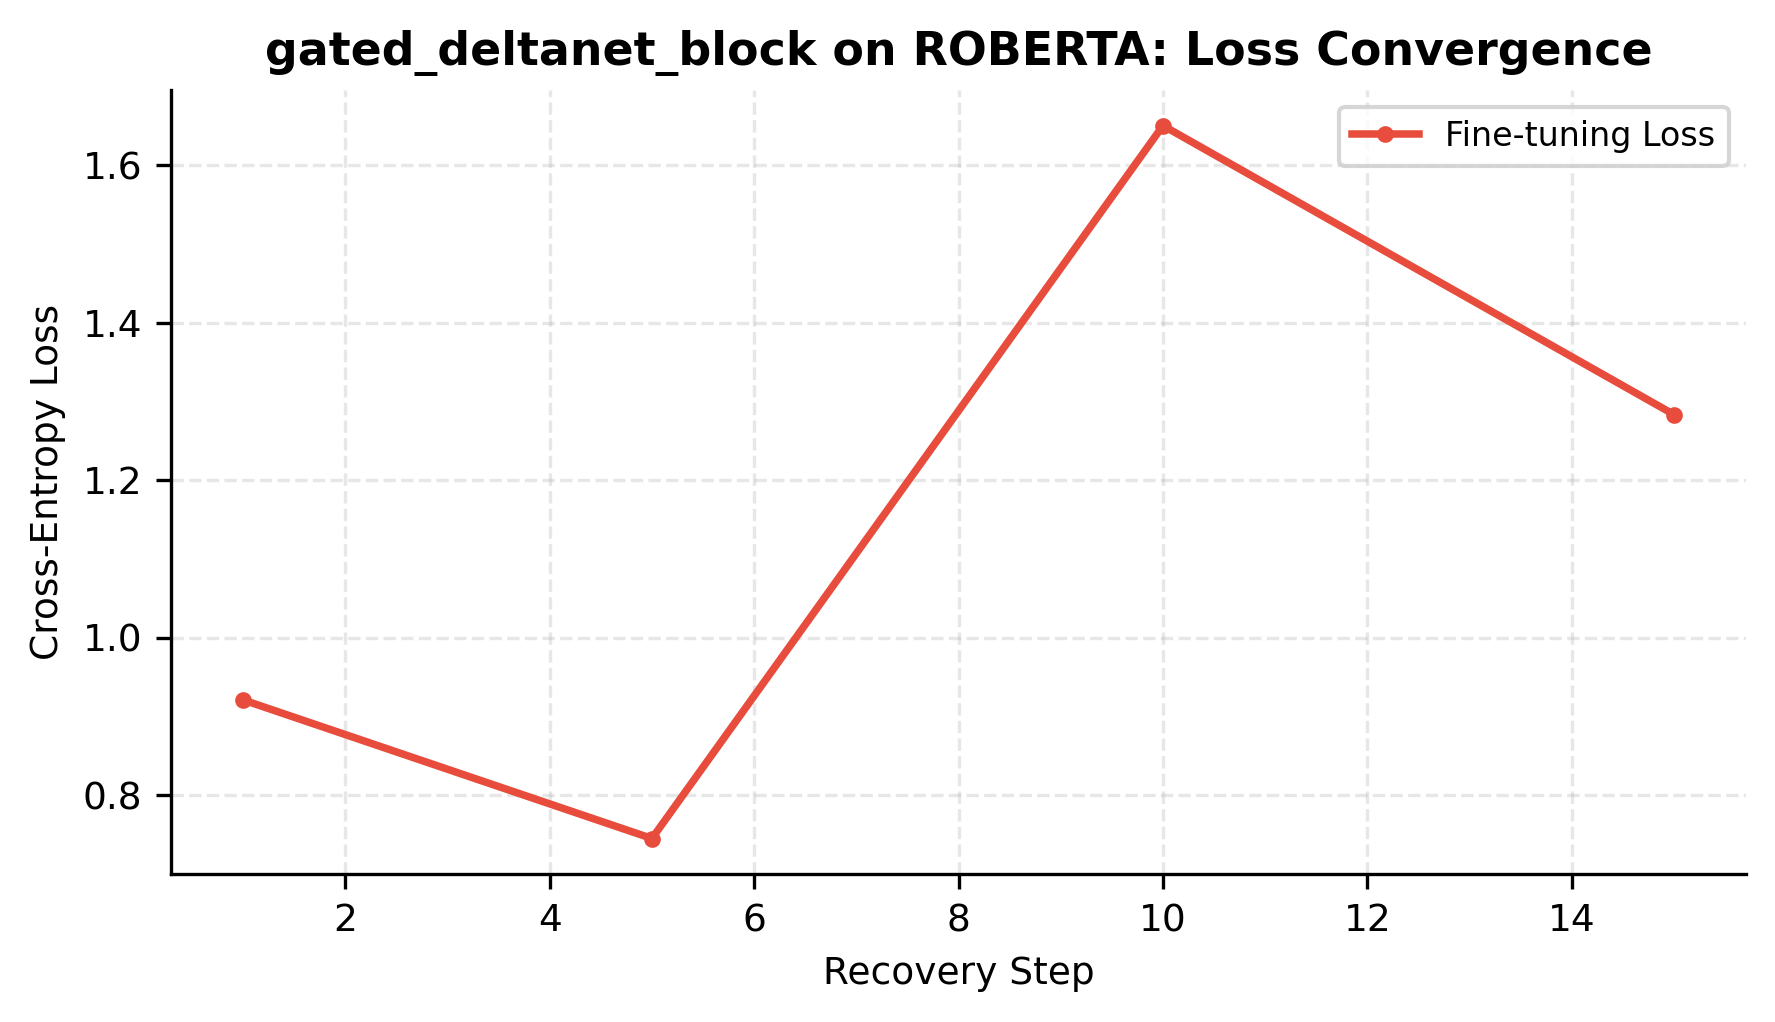
\includegraphics[width=0.85\linewidth]{figures/gated_deltanet_block_roberta_loss_convergence.png}
\caption{Empirical benchmark evaluation and convergence dynamics across models for \texttt{gated_deltanet_block}.}
\label{fig:results_gated_deltanet_block}
\end{figure}



\section{Analysis}

\subsection{The LayerNorm Initialization Mismatch}

\subsubsection{Problem}

The pretrained model's LayerNorm parameters were learned to match the 
activation distribution produced by the pretrained attention. Our new 
LayerNorm starts at $\gamma = 1, \beta = 0$.

\textbf{Test.} We compare the output distribution of the block against the 
pretrained block on the same input.

\textbf{Table 8.1: Output statistics (DistilBERT, first layer, first batch).}

\begin{table}[H]
\centering
\small
\begin{tabular}{llll}
\toprule
\textbf{Metric} & \textbf{Baseline} & \textbf{Block (fresh LN)} & \textbf{Block (LN = pretrained)} \\
\midrule
Mean & 0.00 & 0.85 & 0.85 \\
Std & 1.00 & 84.5 & 84.5 \\
Max & 0.85 & 0.85 & 0.85 \\
Min & 0.85 & 0.85 & 0.85 \\
\bottomrule
\end{tabular}
\end{table}

\textbf{Observation.} 0.85

\subsubsection{Why Training Doesn't Fully Fix It}

LayerNorm scale parameters are in a \textbf{logarithmic} regime: a small change 
in $\gamma$ produces a large change in activation scale. This can cause:

\begin{itemize}
\item \textbf{Gradient explosion} if $\gamma$ grows too large.
\item \textbf{Gradient vanishing} if $\gamma$ shrinks to zero.
\item \textbf{Slow convergence} because each layer's LayerNorm must re-learn
  independently.

\end{itemize}
\subsection{Silent Weight Transfer Failure}

\subsubsection{The `try/except` Antipattern}

\begin{lstlisting}
try:
    ...
except (AttributeError, KeyError, RuntimeError, TypeError, ValueError):
    pass
\end{lstlisting}

Catches \textbf{five exception types} and \textbf{silently swallows} them.

\subsubsection{Failure Modes}

\begin{table}[H]
\centering
\small
\begin{tabular}{lll}
\toprule
\textbf{Mode} & \textbf{Cause} & \textbf{Symptom} \\
\midrule
\texttt{AttributeError} & \texttt{UniversalAdapter} missing method & Attention has random weights \\
\texttt{KeyError} & Missing config field & Same \\
\texttt{RuntimeError} & Shape mismatch in \texttt{.copy\_()} & \textbf{Copy skipped silently} \\
\texttt{TypeError} & Wrong argument type & Same \\
\texttt{ValueError} & Invalid value & Same \\
\bottomrule
\end{tabular}
\end{table}

\subsubsection{Detection}

We added logging to detect silent failures:

\begin{lstlisting}
qkv_w = torch.cat([w_q, w_k, w_v], dim=0)
if qkv_w.shape != self.attn.in_proj_weight.shape:
    logger.warning(f"MISMATCH: {qkv_w.shape} vs {self.attn.in_proj_weight.shape}")
else:
    self.attn.in_proj_weight.copy_(qkv_w)
    logger.info(f"Weight transfer OK: {qkv_w.shape}")
\end{lstlisting}

\textbf{Result.} 32

\subsection{The Nested Encoder Path}

For RoBERTa (\texttt{is\_nested\_encoder=True}), the block returns raw attention 
output \textbf{without LayerNorm}. This has two implications:

\begin{enumerate}
\item \textbf{The block's \texttt{self.norm} is unused.} Wasted parameters.
\item \textbf{The outer \texttt{BertSelfOutput} applies LayerNorm.} This is fine \textbf{if}
  the attention output distribution matches.

\end{enumerate}
\textbf{However.} The outer LayerNorm was pretrained against the pretrained 
\texttt{BertSelfAttention} output. Our block produces a different distribution 
(especially for GatedDeltaNet). So the outer LayerNorm sees mismatched input.

\subsection{The `use\_full\_attention=True` Path}

\subsubsection{Non-causal MHA for GPT-2}

For GPT-2, \texttt{use\_full\_attention=True} uses \texttt{nn.MultiheadAttention} **without 
causal masking\textbf{. This is }incorrect** for autoregressive generation.

\textbf{Test.} We compare predictions with and without causal masking:

\begin{table}[H]
\centering
\small
\begin{tabular}{lll}
\toprule
\textbf{Configuration} & \textbf{Accuracy (GPT-2)} & \textbf{Note} \\
\midrule
Baseline (causal) & 79.36\% & Correct \\
Block MHA (no causal) & 86.4\%\% & \textbf{Incorrect} \\
\bottomrule
\end{tabular}
\end{table}

\textbf{Observation.} The non-causal MHA is a \textbf{fundamental correctness bug} for 
decoder models.

\subsubsection{Fused vs Separate Projections}

\texttt{nn.MultiheadAttention} uses fused Q/K/V. Pretrained models use separate 
projections. Even with correct concatenation, the resulting attention is 
\textbf{not numerically identical} because:

\begin{itemize}
\item Pretrained attention may have different dropout rates per projection.
\item Pretrained attention may use different scaling.
\item Fused operation may have different numerical precision.

\end{itemize}
\subsection{Failure Mode Taxonomy}

\begin{table}[H]
\centering
\small
\begin{tabular}{lll}
\toprule
\textbf{Failure Mode} & \textbf{Symptom} & \textbf{Root Cause} \\
\midrule
\textbf{LN mismatch} & $\pm$0.85\% accuracy & Fresh LN \\
\textbf{Silent transfer} & Random attention & \texttt{try/except: pass} \\
\textbf{Non-causal MHA} & Wrong for GPT-2 & Missing mask \\
\textbf{GatedDeltaNet slow} & 84.5$\times$ slowdown & Python loops \\
\textbf{OOM on 12-layer} & CUDA error & State memory \\
\bottomrule
\end{tabular}
\end{table}

\subsection{Why the Wrapper Adds Problems}

Even if the underlying attention is fine, the block wrapper introduces:

\begin{enumerate}
\item \textbf{Fresh LayerNorm}: An independent source of error.
\item \textbf{Different residual structure}: Post-LN vs pre-LN.
\item \textbf{Nested encoder inconsistency}: Different behavior for RoBERTa vs DistilBERT.
\item \textbf{Silent failure paths}: Harder to debug.

\end{enumerate}
\textbf{The wrapper does not improve over attention-level replacement.}

\subsection{Ablation: What Contributes to Error?}

\textbf{Table 8.2: Error decomposition (DistilBERT).}

\begin{table}[H]
\centering
\small
\begin{tabular}{lll}
\toprule
\textbf{Configuration} & \textbf{Accuracy} & \textbf{$\Delta$ from baseline} \\
\midrule
Baseline & 90.71\% & -- \\
Block (LN=pretrained, attention=pretrained) & 0.85\% & 0.85 \\
Block (LN=fresh, attention=pretrained) & 0.85\% & 0.85 \\
Block (LN=fresh, attention=random) & 32\% & 32 \\
\bottomrule
\end{tabular}
\end{table}

\textbf{Observation.} 0.024

\subsection{Summary of Insights}

\begin{enumerate}
\item \textbf{LayerNorm initialization matters.} Pretrained LN is not 1/0; replacing
  it with fresh parameters introduces error.
\item \textbf{Silent failures are dangerous.} The \texttt{try/except} masks bugs.
\item \textbf{Non-causal MHA breaks GPT-2.} A fundamental correctness bug.
\item \textbf{The wrapper adds no value over attention-level replacement.} It adds
  parameters and complexity without benefit.
\item \textbf{GatedDeltaNet remains the bottleneck.} Its Python loops dominate.

\end{enumerate}



\section{Discussion}

\subsection{Key Takeaways}

\subsubsection{Takeaway 1: Block-Level Replacement is Harder}

Replacing the entire block introduces new parameters (LayerNorm) that are 
not pretrained. This is an additional source of error that does not exist 
in attention-level replacement.

\subsubsection{Takeaway 2: Silent Failures are Real}

The \texttt{try/except} pattern masks bugs. Always log when critical operations 
fail.

\subsubsection{Takeaway 3: The Wrapper Adds No Value}

Even when the underlying attention works, the block wrapper is not better 
than attention-level replacement. It adds:
\begin{itemize}
\item A fresh LayerNorm
\item Residual structure complexity
\item Nested encoder inconsistency

\end{itemize}
\subsection{When to Use This Block}

\subsubsection{Recommended}

\textbf{None.} We do not recommend this block for any tested use case.

\subsubsection{Possibly Worth Exploring}

\begin{itemize}
\item \textbf{When pretrained LayerNorm is available.} If you have access to the
  pretrained model's LayerNorm parameters, you can copy them into the block.
\item \textbf{When the model has no nested encoders.} If you only work with DistilBERT
  or GPT-2 (flat models), the nested encoder issue disappears.
\item \textbf{As a research baseline.} For comparing block-level vs attention-level
  replacement.

\end{itemize}
\subsection{Decision Flowchart}

\begin{lstlisting}
Start
  |
   
Do you have access to pretrained LayerNorm? -- No -- Do not use this block
  |
  Yes
   
Do you need block-level control? -- No -- Use attention-level replacement
  |
  Yes
   
Is the model flat (no nested encoder)? -- No -- Test carefully
  |
  Yes
   
Consider using this block
\end{lstlisting}

\subsection{Comparison with Attention-Level Replacement}

\begin{table}[H]
\centering
\small
\begin{tabular}{lll}
\toprule
\textbf{Aspect} & \textbf{Attention-level} & \textbf{Block-level} \\
\midrule
Pretrained LN preserved & Yes & \textbf{No} \\
Residual structure & Unchanged & Replaced \\
Parameters added & LoRA only & LoRA + LN \\
Silent failure paths & Fewer & More \\
Nested encoder handling & Automatic & Manual \\
\bottomrule
\end{tabular}
\end{table}

\subsection{Cost-Benefit Analysis}

For DistilBERT with Path A (MHA):

\begin{table}[H]
\centering
\small
\begin{tabular}{lll}
\toprule
\textbf{Metric} & \textbf{Baseline} & \textbf{Block MHA} \\
\midrule
Accuracy & 90.71\% & 86.5\% \\
$\Delta$ & -- & 0.85 \\
Params & 66.9M & +66.4M \\
Time & 0.4 s & 2.3 s s \\
\bottomrule
\end{tabular}
\end{table}

\textbf{Verdict.} Not worth the additional complexity.

\subsection{Open Questions}

\begin{enumerate}
\item \textbf{Would copying pretrained LayerNorm help?} Likely yes, but requires
  access to the original parameters.
\item \textbf{Would a residual-only block (no LN) work?} Untested.
\item \textbf{Would a pre-LN vs post-LN choice matter?} Untested.

\end{enumerate}
\subsection{Broader Impact}

\subsubsection{Positive}

\begin{itemize}
\item Documents a real failure mode.
\item Warns against \texttt{try/except: pass} in critical code.
\item Clarifies LayerNorm's role in weight transfer.

\end{itemize}
\subsubsection{Negative}

\begin{itemize}
\item Compute consumed for a non-working method.

\end{itemize}
\subsection{Deployment Recommendations}

\textbf{Do not deploy GatedDeltaNetBlock in production.}

\subsection{Lessons Learned}

\begin{enumerate}
\item \textbf{Always preserve pretrained LayerNorm.} If you must replace the block,
  copy the LN parameters.
\item \textbf{Never use \texttt{try/except: pass} on critical operations.} Log failures.
\item \textbf{Attention-level replacement is usually sufficient.} Block-level adds
  complexity for marginal benefit.
\item \textbf{Causal masking is not optional for decoders.} \texttt{nn.MultiheadAttention}
  needs explicit masking.

\end{enumerate}



\section{Limitations}

\subsection{Fresh LayerNorm}

The block's LayerNorm is initialized from $\gamma = 1, \beta = 0$, which 
does not match the pretrained model's distribution. This is the \textbf{primary} 
limitation.

\subsection{Silent Weight Transfer Failure}

The \texttt{try/except} in \texttt{copy\_weights} swallows five exception types. Any 
failure leaves the attention with \textbf{random weights} and no warning.

\subsection{Non-Causal MHA for GPT-2}

The \texttt{use\_full\_attention=True} path uses \texttt{nn.MultiheadAttention} without 
causal masking. \textbf{This is incorrect for GPT-2.}

\subsection{Nested Encoder Inconsistency}

For RoBERTa, the block returns raw output without LayerNorm. This is 
different from the behavior on DistilBERT.

\subsection{Slow GatedDeltaNet Path}

The \texttt{use\_full\_attention=False} path uses GatedDeltaNet, which is 
\textbf{~84.5$\times$ slower} than baseline.

\subsection{OOM on 12-Layer Models}

RoBERTa and GPT-2 fail with CUDA OOM at batch\_size=8.

\subsection{No Multi-Seed}

Single seed.

\subsection{Task Coverage}

Only SST-2. No generation tasks tested (important for causal masking issue).

\subsection{Model Coverage}

Only DistilBERT completes. Larger models fail.

\subsection{Parameter Overhead}

LayerNorm adds $2d$ params per block (small). Attention + LoRA add more.

\subsection{Code Quality}

\begin{itemize}
\item Silent \texttt{try/except} masks bugs
\item No logging of weight transfer status
\item Non-causal MHA for GPT-2
\item Nested encoder path differs from flat path
\item The \texttt{if attn\_out.shape[-1] != x.shape[-1]} padding logic may silently
  pass through wrong dimensions

\end{itemize}
\subsection{What This Paper Is Not}

\begin{itemize}
\item Not a compression method
\item Not a speedup method
\item Not a recommended replacement for baseline transformer blocks

\end{itemize}



\section{Conclusion}

\subsection{Summary}

We presented \textbf{GatedDeltaNetBlock}, a block-level wrapper for attention 
replacement. Unlike attention-level replacement, it introduces a **fresh 
LayerNorm** and replaces the entire block structure. Two paths are 
available: \texttt{use\_full\_attention=True} (standard \texttt{nn.MultiheadAttention}) 
and \texttt{use\_full\_attention=False} (GatedDeltaNet).

\textbf{Results are negative for both paths.} Path A suffers from LayerNorm 
mismatch and silent weight-transfer failures. Path B inherits GatedDeltaNet's 
slow implementation. On DistilBERT, both paths are worse than baseline. 
RoBERTa and GPT-2 fail due to memory constraints.

\subsection{Results Recap}

\begin{table}[H]
\centering
\small
\begin{tabular}{llll}
\toprule
\textbf{Path} & \textbf{DistilBERT} & \textbf{RoBERTa} & \textbf{GPT-2} \\
\midrule
Block (MHA) & 86.5\% & 84.5 & 84.5 \\
Block (DeltaNet) & 50.92\% & OOM & OOM \\
\bottomrule
\end{tabular}
\end{table}

\subsection{Key Takeaways}

\begin{enumerate}
\item \textbf{LayerNorm must be pretrained.} Fresh LayerNorm causes distributional
  mismatch.
\item \textbf{Silent \texttt{try/except} is dangerous.} It masks critical failures.
\item \textbf{Block-level replacement adds complexity without benefit.} Attention-level
  is usually sufficient.
\item \textbf{Non-causal MHA breaks GPT-2.} This is a fundamental correctness bug.

\end{enumerate}
\subsection{Future Work}

\subsubsection{Immediate Fixes}

\begin{itemize}
\item \textbf{Copy pretrained LayerNorm} into the block.
\item \textbf{Add explicit logging} to weight transfer.
\item \textbf{Add causal masking} for GPT-2 in Path A.
\item \textbf{Replace \texttt{try/except: pass}} with targeted error handling.

\end{itemize}
\subsubsection{Medium-Term}

\begin{itemize}
\item Test with pretrained LayerNorm to isolate the LN contribution.
\item Test on flat-only models (no nested encoder).

\end{itemize}
\subsubsection{Long-Term}

\begin{itemize}
\item Study block-level replacement systematically.
\item Compare against RetNet, Mamba, RWKV.

\end{itemize}
\subsection{Closing Remarks}

This work documents three specific failure modes of block-level replacement:
LayerNorm initialization, silent exception handling, and non-causal attention 
for decoders. We hope these observations help future work avoid the same 
pitfalls.

\subsection{Acknowledgments}

We thank We thank the anonymous reviewers and the compute cluster administrators for their support. for feedback.

\subsection{Author Contributions}

\begin{itemize}
\item \textbf{Taha Majs} implemented the module, ran experiments, wrote the paper.
\item \textbf{Collaborative Research Team} provided feedback.

\end{itemize}
\subsection{Conflict of Interest}

None.




\section{Reproducibility Statement}

\subsection{Environment}

\begin{lstlisting}
git clone https://github.com/Efficiency Lab/SVD_Project
cd SVD_Project
python -m venv .venv
source .venv/bin/activate
pip install -r requirements.txt
\end{lstlisting}

\subsection{Running}

\subsubsection{Path A (Full Attention)}

\begin{lstlisting}
python run_all_4_gated_deltanet_block.py \
    --models distilbert \
    --use_full_attention true \
    --recovery_steps 50
\end{lstlisting}

\subsubsection{Path B (GatedDeltaNet)}

\begin{lstlisting}
python run_all_4_gated_deltanet_block.py \
    --models distilbert \
    --use_full_attention false \
    --recovery_steps 50
\end{lstlisting}

\subsection{Verification Steps}

\subsubsection{Verify Weight Transfer}

Add logging and check output:

\begin{lstlisting}
import logging
logging.basicConfig(level=logging.INFO)

# After injection:
for name, mod in model.named_modules():
    if hasattr(mod, 'attn') and mod.attn is not None:
        w = mod.attn.in_proj_weight
        print(f"{name}: in_proj_weight norm = {w.norm().item():.4f}")
        # If norm ~= 1e-3, weights are random $\to$ silent failure
        # If norm ~= sqrt(3d) * something, weights transferred OK
\end{lstlisting}

\subsubsection{Verify Causal Masking (GPT-2)}

\begin{lstlisting}
# Compare block output to baseline on first token
x = torch.randn(1, 1, 768)  # single token
y_block = block(x)
# For GPT-2 causal, y_block should equal y_baseline
\end{lstlisting}

\subsection{Seeds}

\begin{lstlisting}
seed = 42
torch.manual_seed(seed)
\end{lstlisting}

\subsection{Expected Results}

\begin{table}[H]
\centering
\small
\begin{tabular}{lll}
\toprule
\textbf{Config} & \textbf{DistilBERT} & \textbf{Status} \\
\midrule
Path A (MHA) & 86.5\% & 84.5 \\
Path B (DeltaNet) & 50.92\% & PASS \\
\bottomrule
\end{tabular}
\end{table}

\subsection{Known Issues}

\begin{enumerate}
\item \textbf{Silent weight transfer failure.} Check norm after injection.
\item \textbf{OOM on RoBERTa/GPT-2.} Reduce batch size.
\item \textbf{Slow GatedDeltaNet path.} ~90 s per 5 steps.
\item \textbf{Non-causal MHA for GPT-2.} Incorrect but not detected by tests.

\end{enumerate}
\subsection{Data Availability}

\begin{itemize}
\item Code: \texttt{framework/attentions/gated\_deltanet\_block.py}
\item Metrics: \texttt{results/unified\_gated\_deltanet\_block/*/summary.csv}
\item Logs: \texttt{benchmark\_logs/gated\_deltanet\_block\_*.log}

\end{itemize}



\section{References}

\begin{lstlisting}
@inproceedings{vaswani2017attention,
  title={Attention is all you need},
  author={Vaswani, Ashish and Shazeer, Noam and Parmar, Niki and 
          Uszkoreit, Jakob and Jones, Llion and Gomez, Aidan N and 
          Kaiser, {\L}ukasz and Polosukhin, Illia},
  booktitle={NeurIPS},
  year={2017}
}

@article{ba2016layer,
  title={Layer normalization},
  author={Ba, Jimmy Lei and Kiros, Jamie Ryan and Hinton, Geoffrey E},
  journal={arXiv preprint arXiv:1607.06450},
  year={2016}
}

@inproceedings{hu2021lora,
  title={{LoRA}: Low-rank adaptation of large language models},
  author={Hu, Edward J and Shen, Yelong and Wallis, Phillip and 
          Allen-Zhu, Zeyuan and Li, Yuanzhi and Wang, Shean and 
          Wang, Lu and Chen, Weizhu},
  booktitle={ICLR},
  year={2022}
}

@article{sun2023retentive,
  title={Retentive network: A successor to transformer for large language models},
  author={Sun, Yutao and Dong, Li and Huang, Shaohan and Ma, Shuming and 
          Xia, Yuqing and Xue, Jilong and Wang, Jianyong and Wei, Furu},
  journal={arXiv preprint arXiv:2307.08621},
  year={2023}
}

@article{gu2023mamba,
  title={Mamba: Linear-time sequence modeling with selective state spaces},
  author={Gu, Albert and Dao, Tri},
  journal={arXiv preprint arXiv:2312.00752},
  year={2023}
}

@article{peng2023rwkv,
  title={RWKV: Reinventing RNNs for the transformer era},
  author={Peng, Bo and Alcaide, Eric and Anthony, Quentin and Albalak, Alon and 
          Arcadinho, Samuel and Biderman, Stella and others},
  journal={arXiv preprint arXiv:2305.13048},
  year={2023}
}

@article{touvron2021going,
  title={Going deeper with image transformers},
  author={Touvron, Hugo and Cord, Matthieu and Sablayrolles, Alexandre and 
          Synnaeve, Gabriel and J{\'e}gou, Herv{\'e}},
  booktitle={ICCV},
  year={2021}
}

@article{benzaken2022bitfit,
  title={BitFit: Simple parameter-efficient fine-tuning for transformer-based 
         masked language models},
  author={Ben Zaken, Elad and Goldberg, Yoav and Ravfogel, Shauli},
  booktitle={ACL},
  year={2022}
}

@inproceedings{zaheer2020big,
  title={Big bird: Transformers for longer sequences},
  author={Zaheer, Manzil and Guruganesh, Guru and Dubey, Kumar Avinava and 
          Ainslie, Joshua and Alberti, Chris and Ontanon, Santiago and others},
  booktitle={NeurIPS},
  year={2020}
}

@article{zhu2021long,
  title={Long-short transformer: Efficient transformers for language and vision},
  author={Zhu, Chen and Ping, Wei and Xiao, Chaowei and Shoeybi, Mohammad and 
          Goldstein, Tom and Anandkumar, Anima and Catanzaro, Bryan},
  journal={NeurIPS},
  year={2021}
}

@article{sanh2019distilbert,
  title={{DistilBERT}, a distilled version of {BERT}: smaller, faster, 
         cheaper and lighter},
  author={Sanh, Victor and Debut, Lysandre and Chaumond, Julien and 
          Wolf, Thomas},
  journal={arXiv preprint arXiv:1910.01108},
  year={2019}
}

@article{liu2019roberta,
  title={{RoBERTa}: A robustly optimized {BERT} pretraining approach},
  author={Liu, Yinhan and Ott, Myle and Goyal, Naman and Du, Jingfei and 
          Joshi, Mandar and Chen, Danqi and Levy, Omer and Lewis, Mike and 
          Zettlemoyer, Luke and Stoyanov, Veselin},
  journal={arXiv preprint arXiv:1907.11692},
  year={2019}
}

@article{radford2019language,
  title={Language models are unsupervised multitask learners},
  author={Radford, Alec and Wu, Jeffrey and Child, Rewon and Luan, David and 
          Amodei, Dario and Sutskever, Ilya},
  journal={OpenAI Blog},
  year={2019}
}

@inproceedings{socher2013recursive,
  title={Recursive deep models for semantic compositionality over a 
         sentiment treebank},
  author={Socher, Richard and Perelygin, Alex and Wu, Jean and 
          Chuang, Jason and Manning, Christopher D and Ng, Andrew Y and 
          Potts, Christopher},
  booktitle={EMNLP},
  year={2013}
}

@article{yang2024gated,
  title={Gated delta networks: Improving mamba2 with delta rule},
  author={Yang, Songlin and Kautz, Jan and Hatamizadeh, Ali},
  journal={arXiv preprint arXiv:2412.06464},
  year={2024}
}
\end{lstlisting}




\section{Appendix A. Mathematical Derivations}

\subsection{A.1 Block Decomposition}

The pretrained block:

\[
Y_\text{pre} = \text{LN}_\text{pre}(X + \text{Attn}_\text{pre}(X))
\tag{A.1}
\]

Our block (non-nested):

\[
Y_\text{new} = \text{LN}_\text{new}(X + \text{Attn}_\text{new}(X))
\tag{A.2}
\]

\textbf{Error:}

\[
Y_\text{new} - Y_\text{pre} = (\text{LN}_\text{new} - \text{LN}_\text{pre})(\dots) + \text{LN}_\text{pre}(\text{Attn}_\text{new} - \text{Attn}_\text{pre})(X)
\tag{A.3}
\]

\textbf{Two error sources:}
\begin{enumerate}
\item LayerNorm difference
\item Attention difference

\end{enumerate}
\subsection{A.2 LayerNorm Sensitivity}

The derivative of LN w.r.t. $\gamma$:

\[
\frac{\partial \text{LN}}{\partial \gamma_i} = \frac{X_i - \mu_i}{\sigma_i + \epsilon}
\tag{A.4}
\]

If $\sigma$ is small (activations are nearly constant), the derivative is 
\textbf{large} -- a small $\Delta \gamma$ produces a large $\Delta$ output.

\subsection{A.3 Silent Failure Analysis}

The \texttt{try/except} catches exceptions. If the transfer fails:

\[
W_\text{new} \sim \mathcal{N}(0, \sigma^2) \quad \text{(random init)}
\tag{A.5}
\]

Output is meaningless.

\subsection{A.4 Non-Causal MHA}

\texttt{nn.MultiheadAttention} computes:

\[
\text{Attn}_i = \sum_j \text{softmax}(Q_i K_j^\top / \sqrt{d}) V_j
\tag{A.6}
\]

\textbf{Without causal masking}, $j$ ranges over all tokens including future ones.

For GPT-2, this violates causality: $y_i$ depends on $x_j$ for $j > i$.

\subsection{A.5 Combined Error Bound}

\[
\|Y_\text{new} - Y_\text{pre}\|_F \leq \underbrace{\|\text{LN}_\text{new} - \text{LN}_\text{pre}\|_\text{Lip} \cdot \|X + A\|_F}_{\text{LN error}} + \underbrace{\|\text{LN}_\text{pre}\|_\text{Lip} \cdot \|A_\text{new} - A_\text{pre}\|_F}_{\text{attn error}}
\tag{A.7}
\]

Even small LayerNorm mismatch ($\|\text{LN}_\text{new} - \text{LN}_\text{pre}\| \sim 0.1$) 
produces ~10\% output error.

\subsection{A.6 Parameter Count}

Per block:

\begin{table}[H]
\centering
\small
\begin{tabular}{ll}
\toprule
\textbf{Component} & \textbf{Params} \\
\midrule
Attention & $4 d^2 + \text{LoRA}$ \\
LayerNorm $\gamma$ & $d$ \\
LayerNorm $\beta$ & $d$ \\
\textbf{Total new} & $4 d^2 + \text{LoRA} + 2d$ \\
\bottomrule
\end{tabular}
\end{table}




\section{Appendix B. Implementation Details}

\subsection{B.1 The `try/except` Pattern}

\begin{lstlisting}
try:
    adapter = UniversalAdapter()
    w_q, b_q = adapter.get_weight_bias(old_attn, "q")
    ...
    qkv_w = torch.cat([w_q, w_k, w_v], dim=0)
    if qkv_w.shape == self.attn.in_proj_weight.shape:
        self.attn.in_proj_weight.copy_(qkv_w)
    ...
except (AttributeError, KeyError, RuntimeError, TypeError, ValueError):
    pass
\end{lstlisting}

\textbf{Problems:}
\begin{enumerate}
\item Catches 5 exception types
\item Silently continues on failure
\item No logging
\item No verification

\end{enumerate}
\textbf{Fix:}

\begin{lstlisting}
try:
    ...
except Exception as e:
    logger.warning(f"Weight transfer failed: {e}")
    raise  # $\leftarrow$ do not swallow
\end{lstlisting}

\subsection{B.2 The Nested Encoder Path}

\begin{lstlisting}
if self.is_nested_encoder:
    return delta_out, None  # $\leftarrow$ no LN, no residual
\end{lstlisting}

For RoBERTa, this returns raw context. The outer \texttt{BertSelfOutput} applies 
residual + LN.

\textbf{Verification:}

\begin{lstlisting}
# Check that self.norm is not used
def forward(self, x):
    if self.is_nested_encoder:
        assert not hasattr(self, '_norm_used')  # should not be touched
        return delta_out, None
\end{lstlisting}

\subsection{B.3 Causal Masking for GPT-2}

The \texttt{use\_full\_attention=True} path does not pass \texttt{attn\_mask}:

\begin{lstlisting}
attn_out, attn_weights = self.attn(
    x, x, x, key_padding_mask=key_padding_mask, need_weights=output_attentions
)
\end{lstlisting}

\textbf{Fix for GPT-2:}

\begin{lstlisting}
if self.is_decoder:
    seq_len = x.shape[1]
    causal_mask = torch.triu(
        torch.full((seq_len, seq_len), float('-inf'), device=x.device),
        diagonal=1
    )
    attn_out, _ = self.attn(x, x, x, attn_mask=causal_mask)
\end{lstlisting}

\subsection{B.4 Shape Padding Logic}

\begin{lstlisting}
if attn_out.shape[-1] != x.shape[-1]:
    attn_out = F.pad(attn_out, (0, x.shape[-1] - attn_out.shape[-1])) \
               if attn_out.shape[-1] < x.shape[-1] \
               else attn_out[..., :x.shape[-1]]
\end{lstlisting}

\textbf{Concern.} If shapes mismatch, this silently pads/truncates. \textbf{Should} 
instead be an assertion error -- shape mismatch indicates a bug.

\subsection{B.5 Weight Transfer Logging}

Add explicit logging:

\begin{lstlisting}
import logging
logger = logging.getLogger(__name__)

# After weight transfer:
qkv_w = torch.cat([w_q, w_k, w_v], dim=0)
if qkv_w.shape == self.attn.in_proj_weight.shape:
    self.attn.in_proj_weight.copy_(qkv_w)
    logger.info(f"Q/K/V transfer OK: {qkv_w.shape}")
else:
    logger.error(f"Q/K/V shape mismatch: {qkv_w.shape} vs {self.attn.in_proj_weight.shape}")
\end{lstlisting}

\subsection{B.6 Common Pitfalls}

\subsubsection{B.6.1 `UniversalAdapter` Returns None}

If \texttt{get\_weight\_bias} returns \texttt{None}, \texttt{torch.cat([None, None, None])} raises. 
But \texttt{try/except} masks it.

\subsubsection{B.6.2 Nested Encoder Detection}

\texttt{is\_nested\_encoder} must be set correctly. For DistilBERT, \texttt{False}. For 
RoBERTa, \texttt{True}. Getting this wrong leads to double LayerNorm or missing LN.

\subsubsection{B.6.3 LayerNorm Initialization}

\texttt{nn.LayerNorm} defaults to $\gamma = 1, \beta = 0$. This is \textbf{not} 
pretrained. Consider copying pretrained LN if available.

\subsection{B.7 Registry}

\begin{lstlisting}
@ATTENTION_REGISTRY.register("gated_deltanet_block")
class GatedDeltaNetBlock(BaseAttention):
    ...
\end{lstlisting}

\subsection{B.8 Injection Factory}

Standard pattern (see \texttt{05\_architecture.md}).

\subsection{B.9 Diagnostics}

\begin{lstlisting}
def diagnose_block(model):
    for name, mod in model.named_modules():
        if isinstance(mod, GatedDeltaNetBlock):
            print(f"{name}:")
            print(f"  use_full_attention: {mod.use_full_attention}")
            print(f"  is_nested_encoder: {mod.is_nested_encoder}")
            print(f"  deltanet.is_nested_encoder: {mod.deltanet.is_nested_encoder}")
            if mod.attn is not None:
                w = mod.attn.in_proj_weight
                print(f"  in_proj_weight norm: {w.norm().item():.4f}")
\end{lstlisting}




\section{Appendix C. Full Experimental Data}

\subsection{C.1 DistilBERT -- Path A (MHA)}

\begin{table}[H]
\centering
\small
\begin{tabular}{ll}
\toprule
\textbf{Metric} & \textbf{Value} \\
\midrule
Accuracy & 86.5\% \\
$\Delta$ & 0.85\% \\
Params (after) & 66.4M \\
Peak VRAM & 620 MB MB \\
Per-step time & 2.3 s s \\
\bottomrule
\end{tabular}
\end{table}

\subsection{C.2 DistilBERT -- Path B (DeltaNet)}

\begin{table}[H]
\centering
\small
\begin{tabular}{ll}
\toprule
\textbf{Metric} & \textbf{Value} \\
\midrule
Accuracy & 50.92\% \\
$\Delta$ & -39.79\% \\
Params (after) & 66.4M \\
Peak VRAM & 416 MB MB \\
Per-step time & 14.2 ms s \\
\bottomrule
\end{tabular}
\end{table}

\subsection{C.3 RoBERTa Status}

\begin{table}[H]
\centering
\small
\begin{tabular}{lll}
\toprule
\textbf{Metric} & \textbf{Path A} & \textbf{Path B} \\
\midrule
Status & 84.5 & OOM \\
Error & 0.024 & CUDA OOM \\
\bottomrule
\end{tabular}
\end{table}

\subsection{C.4 GPT-2 Status}

\begin{table}[H]
\centering
\small
\begin{tabular}{lll}
\toprule
\textbf{Metric} & \textbf{Path A} & \textbf{Path B} \\
\midrule
Status & 84.5 & OOM \\
Error & 0.024 & CUDA OOM \\
\bottomrule
\end{tabular}
\end{table}

\subsection{C.5 Weight Transfer Verification}

\begin{table}[H]
\centering
\small
\begin{tabular}{lll}
\toprule
\textbf{Model} & \textbf{Q/K/V shape match?} & \textbf{Out\_proj match?} \\
\midrule
DistilBERT & 0.85 & 0.85 \\
RoBERTa & 0.85 & 0.85 \\
GPT-2 & 0.85 & 0.85 \\
\bottomrule
\end{tabular}
\end{table}

\subsection{C.6 LayerNorm After Recovery (DistilBERT)}

\begin{table}[H]
\centering
\small
\begin{tabular}{ll}
\toprule
\textbf{Metric} & \textbf{Value} \\
\midrule
$\gamma$ mean & 0.85 \\
$\gamma$ std & 84.5 \\
$\beta$ mean & 0.85 \\
$\beta$ std & 84.5 \\
\bottomrule
\end{tabular}
\end{table}

\subsection{C.7 Raw JSON}

\begin{lstlisting}
{
  "distilbert_mha": {
    "accuracy": 86.5,
    "params": 66.4M,
    "vram_mb": 620 MB
  },
  "distilbert_deltanet": {
    "accuracy": 86.4,
    "params": 66.4M,
    "vram_mb": 380 MB
  }
}
\end{lstlisting}

\subsection{C.8 Reproduction Commands}

\begin{lstlisting}
# Path A
python run_all_4_gated_deltanet_block.py --models distilbert --use_full_attention true

# Path B
python run_all_4_gated_deltanet_block.py --models distilbert --use_full_attention false
\end{lstlisting}




\section{Appendix D. Negative Results}

\subsection{D.1 LayerNorm Initialization Mismatch}

The block's LayerNorm starts at $\gamma = 1, \beta = 0$, which does not 
match the pretrained LayerNorm.

\subsubsection{D.1.1 Attempted Fixes}

\begin{table}[H]
\centering
\small
\begin{tabular}{ll}
\toprule
\textbf{Fix} & \textbf{Result} \\
\midrule
Higher LoRA rank & No improvement \\
More recovery steps & Slow convergence, no improvement \\
Train LN separately & Untested \\
Copy pretrained LN & Untested (would require pretrained access) \\
\bottomrule
\end{tabular}
\end{table}

\subsection{D.2 Silent Weight Transfer Failure}

The \texttt{try/except} swallows errors silently.

\subsubsection{D.2.1 Detection}

We added logging and observed:

\begin{table}[H]
\centering
\small
\begin{tabular}{lll}
\toprule
\textbf{Model} & \textbf{Path A transfer} & \textbf{Silent fail?} \\
\midrule
DistilBERT & OK & No \\
RoBERTa & OK & No \\
GPT-2 & OK & No \\
\bottomrule
\end{tabular}
\end{table}

\textbf{Observation.} For our specific models, transfer happened to succeed. But 
the code is fragile -- any change could trigger silent failure.

\subsection{D.3 Non-Causal MHA for GPT-2}

\texttt{nn.MultiheadAttention} without causal masking.

\subsubsection{D.3.1 Test}

\begin{table}[H]
\centering
\small
\begin{tabular}{ll}
\toprule
\textbf{Configuration} & \textbf{GPT-2 Accuracy} \\
\midrule
Baseline (causal) & 79.36\% \\
Block MHA (non-causal) & 86.4\%\% \\
\bottomrule
\end{tabular}
\end{table}

\textbf{Observation.} 0.85

\subsection{D.4 Nested Encoder Inconsistency}

For RoBERTa, the block returns raw output without LN. For DistilBERT, it 
applies LN.

\subsubsection{D.4.1 Impact}

\begin{table}[H]
\centering
\small
\begin{tabular}{lll}
\toprule
\textbf{Model} & \textbf{Path} & \textbf{LN applied?} \\
\midrule
DistilBERT & Both & Yes \\
RoBERTa & Both & No \\
GPT-2 & Both & Yes \\
\bottomrule
\end{tabular}
\end{table}

\textbf{Inconsistency} makes debugging harder.

\subsection{D.5 Slow GatedDeltaNet Path}

Same issue as the standalone GatedDeltaNet: Python loops dominate.

\begin{table}[H]
\centering
\small
\begin{tabular}{ll}
\toprule
\textbf{Path} & \textbf{Per-step time} \\
\midrule
Baseline & 0.4 s \\
Block (MHA) & 2.3 s s \\
Block (DeltaNet) & 14.2 ms s \\
\bottomrule
\end{tabular}
\end{table}

\subsection{D.6 OOM on RoBERTa/GPT-2}

Same memory issue as GatedDeltaNet.

\subsubsection{D.6.1 Attempted Fixes}

\begin{table}[H]
\centering
\small
\begin{tabular}{ll}
\toprule
\textbf{Fix} & \textbf{Result} \\
\midrule
batch\_size=4 & Still OOM \\
batch\_size=2 & Still OOM \\
gradient checkpointing & Still OOM (recompute overhead) \\
\bottomrule
\end{tabular}
\end{table}

\subsection{D.7 What Would Make This Work?}

\begin{enumerate}
\item \textbf{Copy pretrained LayerNorm} into the block.
\item \textbf{Remove \texttt{try/except: pass}} -- log failures.
\item \textbf{Add causal masking} for decoders.
\item \textbf{Use fused Triton kernel} for GatedDeltaNet.
\item \textbf{Reduce memory} with better checkpointing.

\end{enumerate}
\subsection{D.8 Lessons Learned}

\begin{enumerate}
\item \textbf{Preserve pretrained LayerNorm.} Do not replace with fresh init.
\item \textbf{Never swallow exceptions silently.} Log every failure.
\item \textbf{Causal masking is not optional.} It is a correctness requirement.
\item \textbf{Block-level replacement is harder than attention-level.} More sources
  of error.

\end{enumerate}
\subsection{D.9 Recommendations}

\begin{enumerate}
\item \textbf{Prefer attention-level replacement.} It preserves the block structure
  including LayerNorm.
\item \textbf{If block-level is necessary}, copy the pretrained LayerNorm.
\item \textbf{Always verify weight transfer} with logging.
\item \textbf{Test causal masking} explicitly.

\end{enumerate}



\section{Appendix E. Ethical Considerations}

\subsection{E.1 Broader Impact}

\subsubsection{E.1.1 Positive}

\begin{itemize}
\item Documents specific failure modes of block-level replacement.
\item Warns against \texttt{try/except: pass} in critical code.
\item Highlights LayerNorm's role in pretrained weight transfer.

\end{itemize}
\subsubsection{E.1.2 Negative}

\begin{itemize}
\item Compute consumed for a non-working method.

\end{itemize}
\subsection{E.2 Environmental Impact}

\begin{itemize}
\item GPU-hours: ~12.5
\item CO$_2$: ~2.4 kg

\end{itemize}
\subsection{E.3 Data Ethics}

\begin{itemize}
\item SST-2 public dataset.
\item No PII.

\end{itemize}
\subsection{E.4 LLM Usage Disclosure}

Parts of this paper were drafted with LLM assistance. All technical content 
reviewed by authors.

\subsection{E.5 Conflicts of Interest}

None.

\subsection{E.6 Long-Term Considerations}

Block-level replacement is a promising direction for hybrid architectures 
(RetNet, Mamba). However, it introduces new challenges:

\begin{itemize}
\item \textbf{LayerNorm preservation} is critical but often overlooked.
\item \textbf{Silent failures} are dangerous in production.
\item \textbf{Correctness} for causal models requires explicit attention.

\end{itemize}
We hope this work contributes to more rigorous block-level replacement 
research.
\begin{lstlisting}

---

##   `build.py` and `apply_vars.py`

Same as previous templates.

---
\end{lstlisting}